
\documentclass{article}
%************************************
\usepackage[utf8]{inputenc} 
\usepackage[total={18cm,24cm},centering]{geometry} 
\usepackage{natbib} 
\setcitestyle{super,open={},close={},citesep={,}} 

\usepackage[colorlinks,citecolor=blue,linkcolor=blue,urlcolor=blue]{hyperref} 
\usepackage{graphicx} 
\usepackage{tabularx} 
\usepackage{titlesec}
\titleformat*{\section}{\bf\centering\MakeUppercase}
\usepackage{authblk}

\newcommand\blankfootnote[1]{
  \begingroup
  \renewcommand\thefootnote{}\footnote{#1}
  \addtocounter{footnote}{-1}
  \endgroup
}

\title{\textbf{Utilización Comparativa de Entity Framework y NHibernate}}

\author[1]{Brian Anco} 
\author[2]{Ericka Martínez}
\author[3]{José Contreras}

\affil[1]{Universidad Privada de Tacna, Perú. Email: briancoc@upt.pe}
\affil[2]{Universidad Privada de Tacna, Perú. Email: erimartinezy@upt.pe}
\affil[3]{Universidad Privada de Tacna, Perú. Email: joscontrerasm@upt.pe}

\date{}

%***************************************************************************************

\begin{document}
\maketitle

\begin{abstract}
     (Mapeo Objeto relacional) es la técnica de programación que nos permite transformar los datos entre el sistema de tipos utilizados en un lenguaje de programación orientado a objetos y el utilizado en una base de datos relacional, utilizando un motor de persistencia. Lo que da como resultado una base de datos orientada a objetos virtual sobre la base de datos relacional. Esta transformación permite el uso de las bondades de la programación orientada a objetos. Los ORM nacieron a mediados de la década del 90, se hicieron masivos a partir de la masificación de Java. Por esta razón, los frameworksmás populares hoy en día en .NET son adaptaciones del modelo pensado en Java. Uno de los componentes de OMR más utilizado, por no decir el más utilizado es HIBERNATE, surgido del ambiente JAVA y llevado al uso del framework.NET con la versión NHIBERNATE.
\end{abstract}

\begin{abstract}
(Relational Object Mapping) is the programming technique that allows us to transform the data between the type system used in an object-oriented programming language and the one used in a relational database, using a persistence engine. Which results in a virtual object-oriented database on the relational database. This transformation allows the use of the benefits of object-oriented programming. The ORMs were born in the mid-90s, they became massive from the massification of Java. For this reason, the most popular frameworks today in .NET are adaptations of the model thought in Java. One of the most used OMR components, if not the most widely used, is HIBERNATE, which emerged from the JAVA environment and led to the use of the .NET framework with the NHIBERNATE version.  
\end{abstract}


\section{Introducción}
 El mapeo objeto-relacional es una técnica de programación para convertir datos entre el sistema de tipos utilizado en un lenguaje de programación orientado a objetos y el utilizado en una base de datos relacional. En la práctica esto crea una base de datos orientada a objetos virtual, por sobre la base de datos relacional. Esto posibilita el uso de las características propias de la orientación a objetos (básicamente herencia y polimorfismo).
\newpage
\section{Desarrollo}
\subsection{Object Relational Mapping (ORM)}
Es un modelo de programación en el cual las tablas de la base de datos se convierten en entidades, de esta manera el ORM puede acceder a la tabla en la base de datos, manipularla y realizar las acciones insertar, actualizar, eliminar listar. El ORM se encarga de traducir nuestra instrucción, en el lenguaje de programación que estemos utilizando, a una instrucción válida y correctamente escrita al motor de base de datos indicado. La interración entre el programador y la base de datos desaparece, únicamente existirá la programación entre el programador y el ORM. Esto facilita tareas de migración, brindando ventajas como la velocidad de uso y provee una capa de seguridad adicional de acceso a datos.

\subsection{Entity Framework}
\subsubsection{Definición}
Creado por Microsoft, Entity Framework es un potente ORM que facilita el trabajo del mapeo a las entidades, y facilita la implementación de la capa de datos utilizando LinQ. Un ORM nos permite mantener el diseño de nuestra base de datos, esto hace que la aplicación sea mantenible y extensible. Algunas de sus principales desventajas, son la posiblidad de afectar el rendimiento de la aplicación y que debemos aprender una nueva expresión para el ORM.\\Entity Framework automatiza la operación estándar de CRUD y permite a los desarrolladores trabajar con datos en forma de objetos, sin tener que preocuparse de las tablas y columnas de la base de datos.
\subsubsection{Aplicación}
Ejemplificaremos la aplicación de Entity Framework sobre un proyecto desarrollado en C#. La descarga e instalación de nuestro ORM se realizará directamente desde Visual Studio, con el administrador de NuGets del proyecto.

\begin{figure}[ht]
    \centering     
    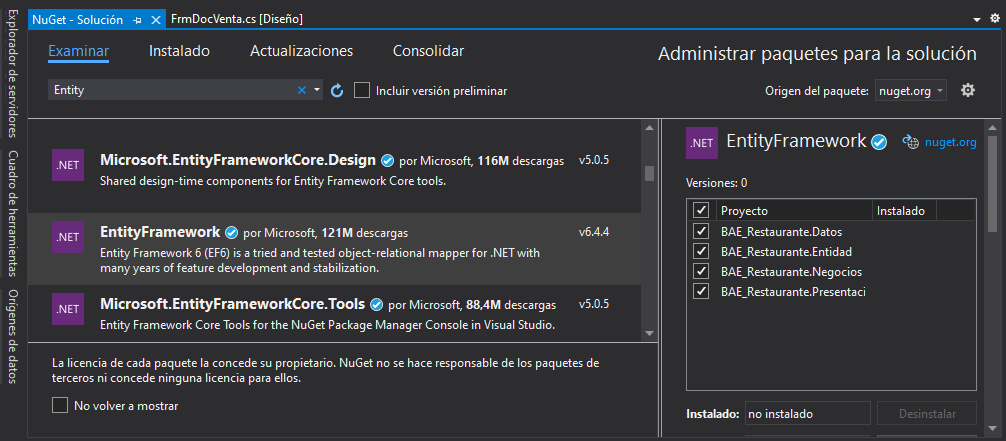
\includegraphics[height=4cm]{images/B1.png}
    \caption{Descarga e instalación de Entity Framework en Visual Studio 2019.}
    \label{fig:BiasVoltage}
\end{figure}
\begin{figure}[ht]
    \centering     
    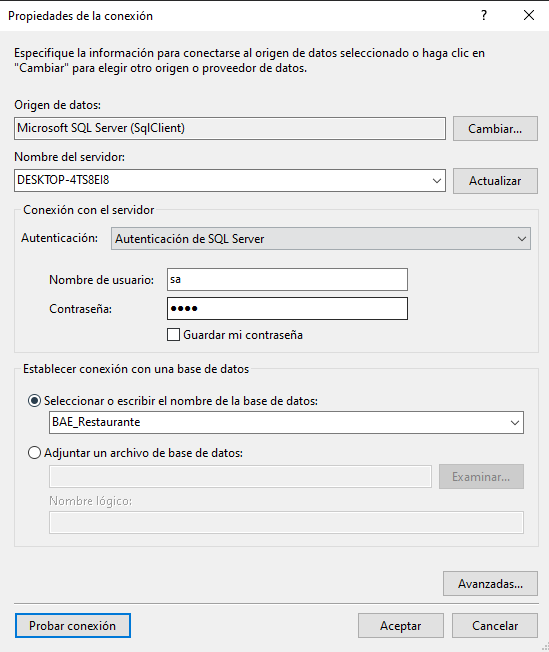
\includegraphics[height=6cm]{images/B4.png}
    \caption{Definición de la cadena de conexión.}
    \label{fig:BiasVoltage}
\end{figure}
A continuación seleccionamos los objetos y la configuración de la base de datos.
\begin{figure}[ht]
    \centering     
    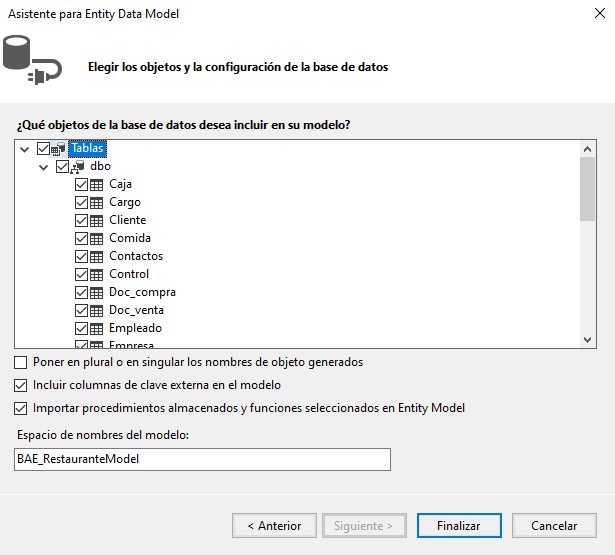
\includegraphics[height=9cm]{images/B6.png}
    \caption{Objetos y configuración de la base de datos.}
    \label{fig:BiasVoltage}
\end{figure}

Una vez terminado el proceso, podremos ver las tablas mapeadas, que son una representación del Entity Framework de lo que hemos mapeado.
\begin{figure}[ht]
    \centering     
    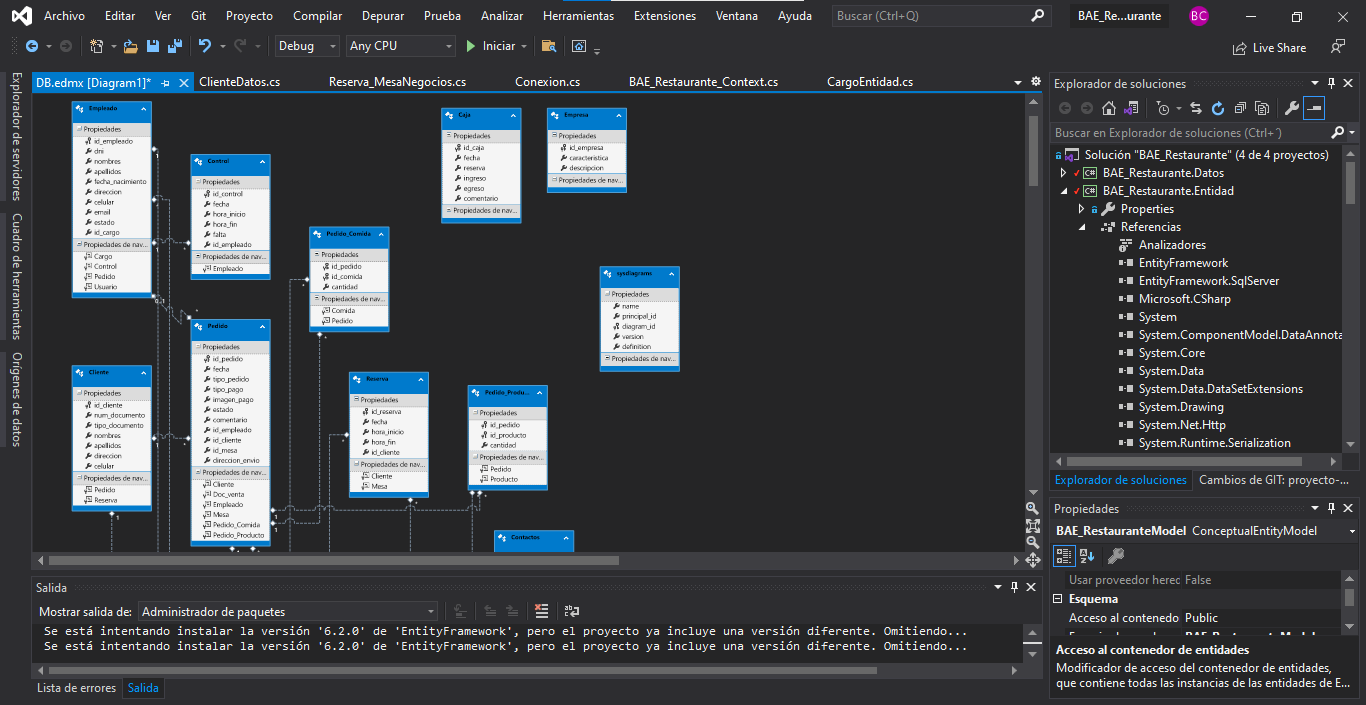
\includegraphics[height=7cm]{images/B7.png}
    \caption{Mapeo de la base de datos BAE Restaurante.}
    \label{fig:BiasVoltage}
\end{figure}

Para reflejar este resultado, modificaremos el código de nuestro formulario Clientes para trabajar con nuestro ORM y LINQ utilizando el siguiente código:
\newpage
\begin{figure}[ht]
    \centering     
    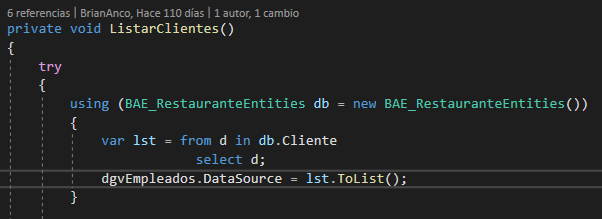
\includegraphics[height=5cm]{images/B8.png}
    \caption{Listar tabla de Clientes.}
    \label{fig:BiasVoltage}
\end{figure}
\subsection{NHibernate }
\subsubsection{Definición}
NHibernate es la conversión de Hibernate de lenguaje Java a C# para su integración en la plataforma .NET. NHibernate es software libre, distribuido bajo los términos de la LGPL (Licencia Pública General Menor de GNU).
\\\\Al usar NHibernate para el acceso a datos el desarrollador se asegura de que su aplicación es agnóstica en cuanto al motor de base de datos a utilizar en producción, pues NHibernate soporta los más habituales en el mercado: MySQL, PostgreSQL, Oracle, MS SQL Server, etc. Sólo se necesita cambiar una línea en el fichero de configuración para que podamos utilizar una base de datos distinta.

\subsubsection{Aplicación}
Utilizando como base nuestro sistema de gestión para un restaurante "BAE-RESTAURANTE". Abriremos Visual Studio 2019 y procederemos a abrir el proyecto.
Entonces, nos dirigiremos a la sección de Referencias -> Administrar paquetes de NuGet.
Descargaremos el paquete seleccionado y, en este caso, la versión 4.1.1.4000, tal como se indica en la siguiente imagen.

\begin{figure}[ht]
    \centering     
    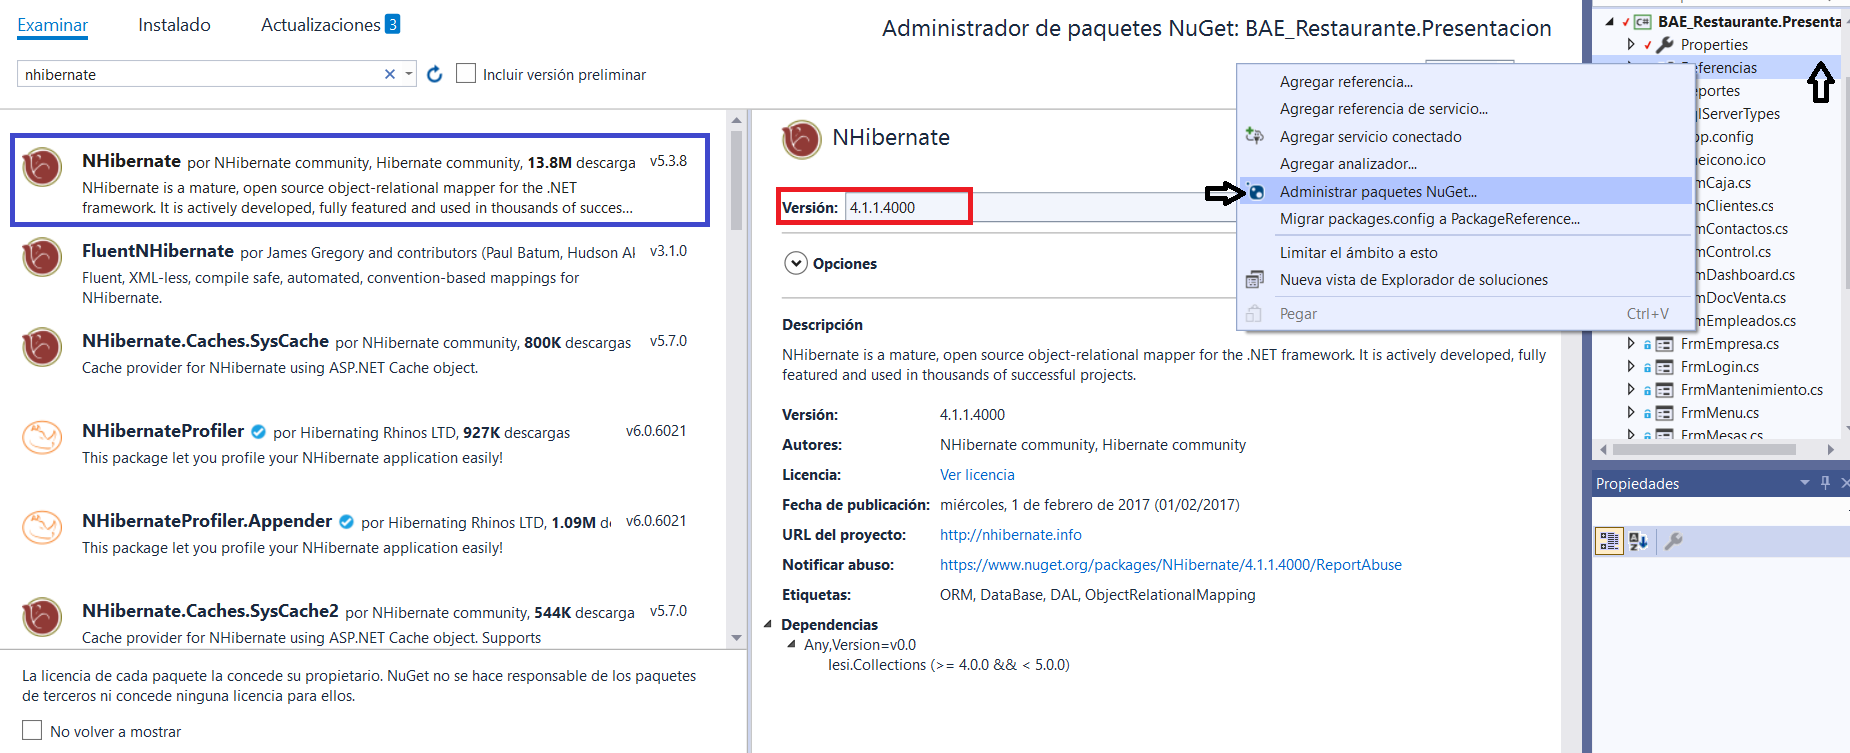
\includegraphics[height=6.5cm]{images/E-figura1.png}
    \caption{Descarga del paquete NHibernate.}
    \label{fig:BiasVoltage}
\end{figure}

\\\\Seguidamente se instalará el paquete FluentNHibernate en la version 2.0.2 para que en lugar de escribir documentos XML. Con la ayuda de Fluent NHibernate, puede escribir asignaciones en código C # fuertemente tipado.
\begin{figure}[ht]
    \centering     
    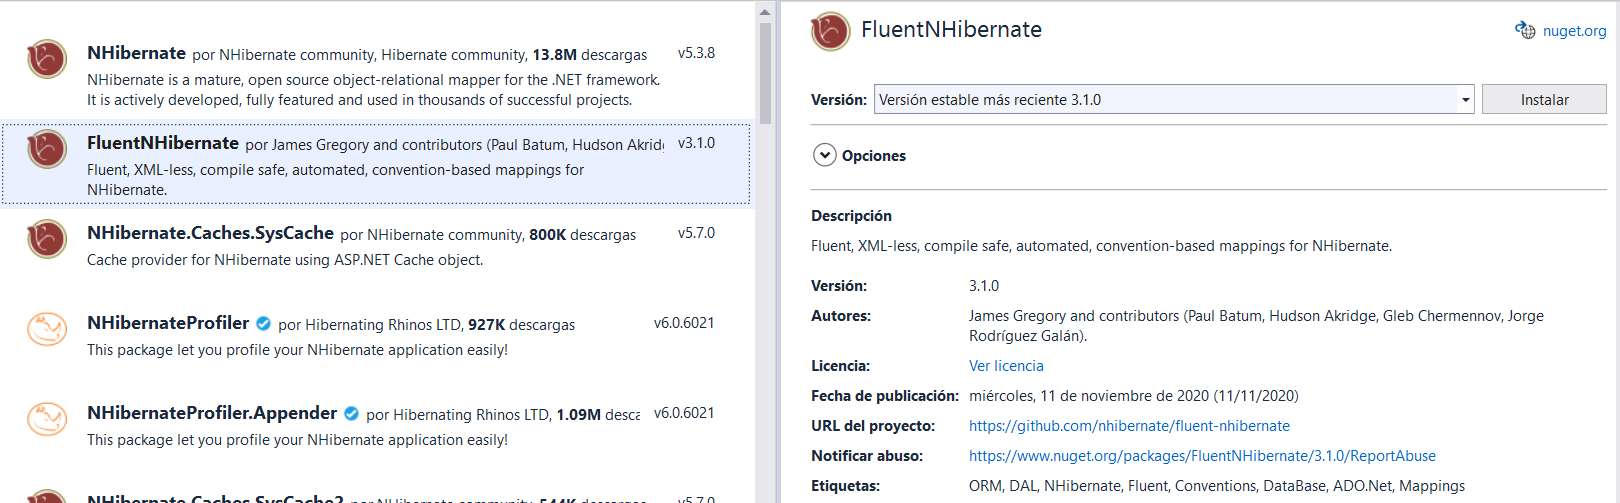
\includegraphics[height=4cm]{images/E-figura2.png}
    \caption{Descarga del paquete NHibernate.}
    \label{fig:BiasVoltage}
\end{figure}
Se realizará la configuración correspondiente para conectarlo a la base de datos en App.config
\\\\
En este caso el sistema se trabaja en 3 capas: Presentación, Modelo y Mapeo. Se creará un "Mapping" para cada modelo, donde, se hace referencia a cada tabla creada en la base de datos.

Utilizando NHibernate vemos claramente la diferencia del uso tradicional al uso de ORM.
\begin{figure}[ht]
    \centering     
    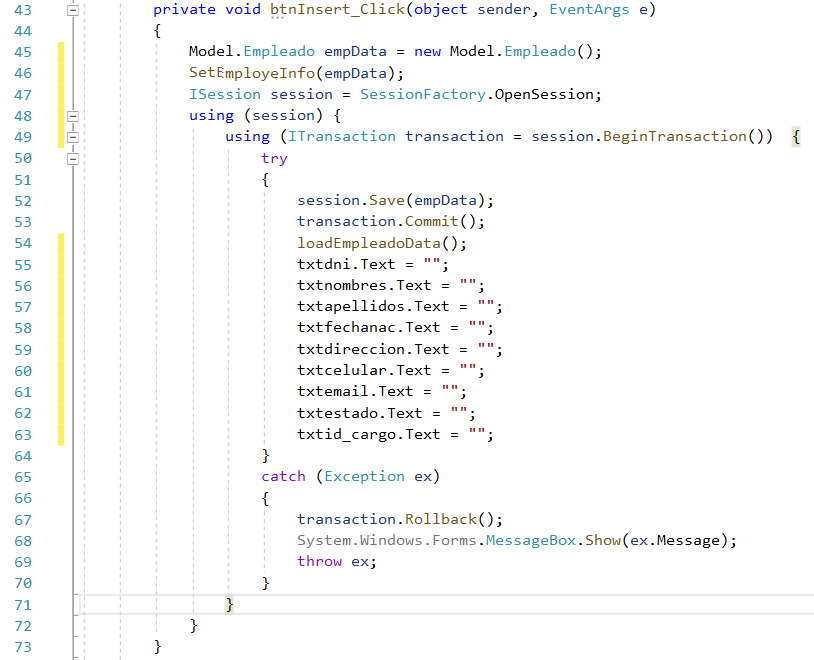
\includegraphics[height=8cm]{images/E-figura5.png}
    \caption{Insertar Empleados.}
    \label{fig:BiasVoltage}
\end{figure}
\begin{figure}[ht]
    \centering     
    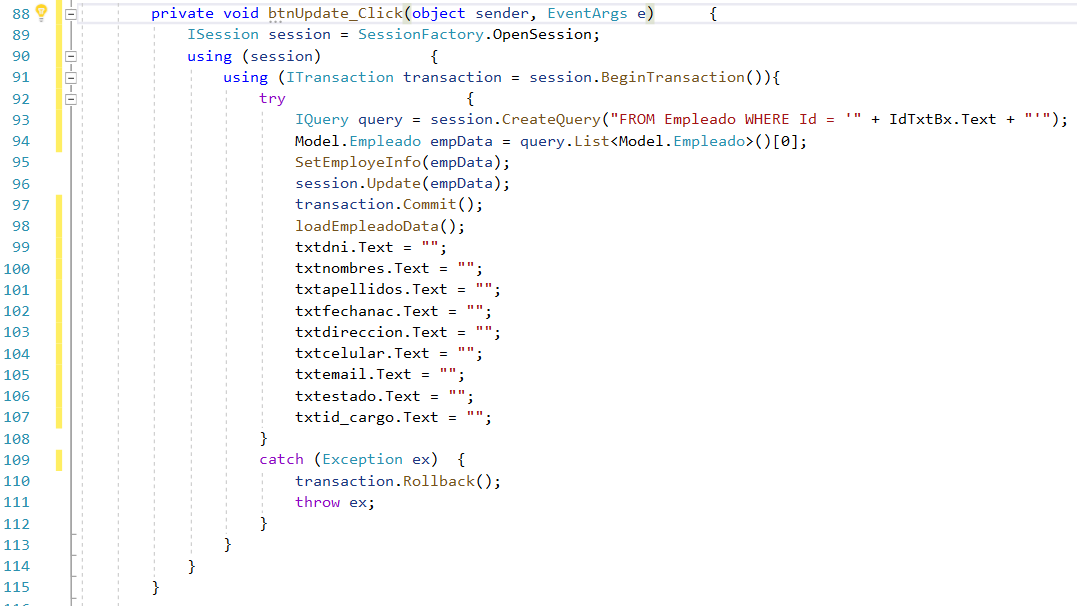
\includegraphics[height=7cm]{images/E-figura6.png}
    \caption{Actualizar Empleados.}
    \label{fig:BiasVoltage}
\end{figure}
\begin{figure}[ht]
    \centering     
    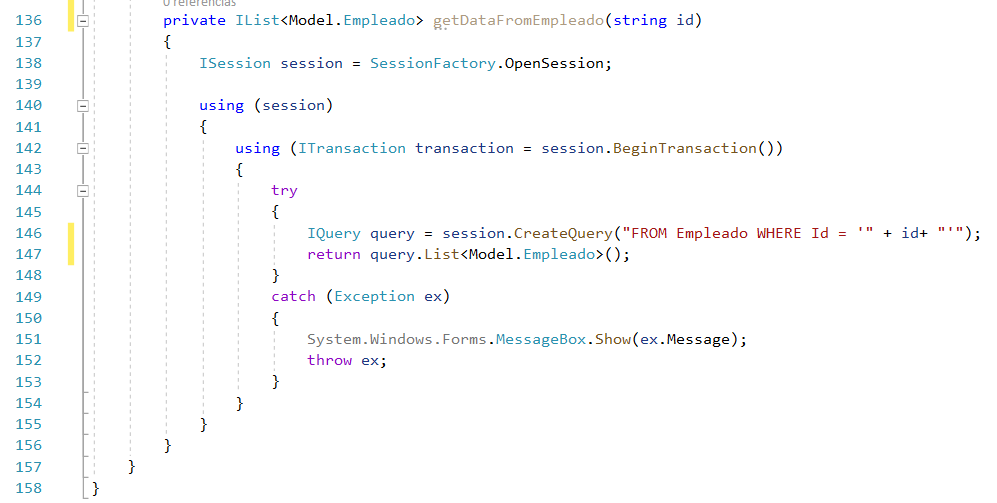
\includegraphics[height=7cm]{images/E-figura7.png}
    \caption{Listar Empleados.}
    \label{fig:BiasVoltage}
\end{figure}
\newpage
\subsection{Comparación entre Entity Framework y NHibernate}
Para poder realizar una comparación entre Entiy Framework y NHibernate, dividiremos esta sección en pequeñas partes donde observaremos a cada ORM desde diferentes puntos de vista
\subsubsection{Plataformas}
NHibernate es compatible con .NET 4 y versiones superiores, compatible con .NET Core. No hay planes para que admita fuentes de datos que no sean bases de datos relacionales.
EF se ejecuta en cualquier plataforma que permita .NET Core. Se basa en un modelo de proveedor que puede funcionar con cualquier tipo de fuente de datos, no solo con las relacionales.

\subsubsection{Arquitectura}
NHibernate se distribuye a través de NuGet como una única DLL, sin otras dependencias a menos que necesitemos conjuntos ordenados, donde también necesitamos Iesi.Collections. Todo está integrado. Necesita .NET Framework completo o .NET Core.
Entity Framework Core, por otro lado, consta de múltiples DLL, que vienen en muchos paquetes NuGet. Lo bueno es que las dependencias de NuGet se incorporan según sea necesario, por lo que, para SQL Server, solo necesita obtener Microsoft.EntityFrameworkCore.SqlServer. Se dirige a .NET Core, por supuesto.

\subsubsection{Configuración y Mapeos}
Entity Framework Core utiliza una configuración fluida (basada en código) y asignaciones fluidas o basadas en atributos. Las convenciones integradas no se pueden reemplazar ni agregar en este momento.
NHibernate tiene tanto XML como configuración y mapeos fluidos. También ofrece asignaciones de atributos a través del proyecto complementario NHibernate Attributes . Las convenciones personalizadas son muy poderosas en NHibernate, EF Core todavía no las tiene, y esto es algo en lo que NHibernate es mejor en este momento.
Ambos necesitan mapeos, en cualquier forma. Ambos pueden mapear miembros, propiedades o campos no públicos. Además, ambos tienen la noción de tipos de valor (entidades de propiedad en EF, componentes en NHibernate). NHibernate puede asignar una propiedad o campo a un comando SQL personalizado.
Además, ambos admiten propiedades de sombra, es decir, entidades que forman parte del esquema de la base de datos, pero que no están asignadas al modelo de clase. Con EF Core, incluso podemos consultarlos.

\section{Conclusiones}
El uso de la herramienta ORM, permite la correspondencia lógica y natural entre modelo relacional a modelo de objetos. Optimizando recursos de tiempo y rapidez, adicionalmente minimizando los errores debido a que es un proceso automático donde la intervención del programador es menor

\section{Bibliografía}
Rodriguez, Gonzalez y Gomez, M. (2007). Estructura de datos, un enfoque moderno. Recuperado de https://elibro.net /es/lc/bibliotecaupt/titulos/62039
\\\\Schneider, M. (2015). Data Structures for Databases. Recuperado de https://www.researchgate.net/profile/Markus-Schneider-3/publication/241149187_Data_Structures_for_Databases/links/54a56d860cf257a63608cebf/Data-Structures-for-Databases.pdf



\bibliographystyle{ieeetr}
\bibliography{references}

\end{document}
